\section{Change Metrics}
\label{sec:changemetrics}

In this section, we give some background information on change metrics, and how there are computed using version control systems. Then, we explain using a concrete example how renaming can affect the values of these metrics.

\subsection{Computing Change Metrics}

As explained in \secref{intro}, change metrics are computed from the sequence of versions of a software artifact. Since projects are almost stored in version control systems (VCSs), we described how the software artifacts are stored in such VCSs. A VCS generally considers a project as a set of files. It stores every version of the project since the beginning of its development. Several metadata are attached to each version: the identity of the developer that committed it, the files that have been added, modified or deleted since the previous version, and its date.

To recognize the files across the versions, VCSs use their absolute path in the repository. It means that as soon as a file is moved or renamed, the VCS will detect it as the deletion of the file with the old absolute path, and the addition of the file with the new absolute path. Although several VCSs provide commands or algorithms to record renamed and moved files, only Git handles this problem out of the box.

Computing change metrics is a straightforward process. Change metrics are computed in a period of time. Such period is represented as a sequence of versions in the VCS. Change metrics are usually computed for every file present at the last version of the period. Then the sequence of versions is browsed backwards until it reaches the first version or the creation of the file. When the version metadata indicates that the file of interest have been modified or created, this file version is included in the sequence of versions concerning the file. Then the change metric is computed using this sequence of file versions.

\subsection{Renaming and Change Metrics}

\figref{example} shows an example of a simple software project history. This project contains only one file, \texttt{Test.php}, which is renamed in the last version to \texttt{Hello.php}. As an example of change metrics we will use \emph{code churn}, \emph{number of developers} and \emph{number of modifications}. The definition of number of developers and number of modifications is straightforward. Code churn correspond to the number of lines added and deleted in the file since its initial version.

\begin{figure}[t]
	\centering
	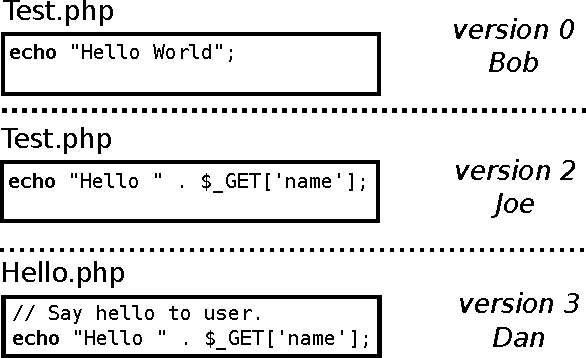
\includegraphics[width=0.8\linewidth,keepaspectratio]{data/figures/example.pdf}
	\caption{Example of a project history. The project is composed of only one file \texttt{Test.php} which is renamed to \texttt{Hello.php} in the last version.}
	\label{fig:example}
\end{figure}

If renaming is not taken into account, the last version of the project of \figref{example} contains only one file, that has only one version. Therefore its code churn is $2$ (it has 2 lines of codes), and the number of developers and modification is $1$. However, if renaming is taken into account, the last version of the project contains one file that has $3$ versions. In this case the code churn is $4$ ($1$ for version 1, $2$ for version 2 and $1$ for version $3$). The number of developers and modifications are $3$. Therefore this small example shows the importance of taking renaming into account.
